\chapter{Geometrical quantum mechanics}
\section{Kahler manifolds}

\section{From the projective Hilbert space to state manifolds}

\subsection{Projective Hilbert space}
Consider the Hilbert space $\H$ to be a space of \emph{bare states} and $\mathcal{S}$ to be the space of \emph{normalized bare states}. Physical observables are related to the \emph{space of rays}, defined as $\PH\coloneqq \mathcal{H}/U(1)$, for the factorization by elements of $U(1)$. This group consists of unitary transformations $e^{i\phi}$ for $\phi\in\R$, defining gauge symmetry between quantum states. $\PH$ is then considered to be the \emph{space of pure states}. For the sake of generality, let's not normalize our vectors yet, which would lead to the \emph{space of unnormalized pure physical states}. 

It can be shown, that $\PH$ is of a K\"ahler structure, meaning it has two non-degenerate sesquilinear\footnote{We are in physics, so complex conjugated is the first input of the 2-form.} 2-forms embedded along with operator complex unit
$$(J, G, \Omega),$$
such that
\begin{equation}
    J^2=\Id
\end{equation}
and any bracket of $\ket{\psi_1},\ket{\psi_2}\in \PH$ can be decomposed into real and imaginary part\citep{ashtekar_geometrical_1997}
\begin{equation}
    \braket{\psi_1|\psi_2}=\frac{1}{2}G(\psi_1,\psi_2)-\frac{i}{2}\Omega(\psi_1,\psi_2).
    \label{eq:quantumProd}
\end{equation}

From braket sesquilinearity goes that $G$ is symmetric and $\Omega$ antisymmetric form, thus they can be uniquely written into one 2-form called \emph{Fubini-Study metric} with property
\begin{equation}
    G=\Re Q ;\qquad \Omega=\Im Q.
\end{equation}

Because $\braket{\psi_1|\psi_2}\in[0,1]$ we say, that the metric is measuring the geodesic distance on the Bloch sphere. Here if we define
\begin{equation}
    |\braket{\psi_1|\psi_2}|=\cos^2 \frac{\theta}{2},
\end{equation}
we get $\d \theta= 2\d s=2\sqrt{|g_{\mu\nu}\d \llambda^\mu\d \llambda^\nu|}$, see \citet{cheng_quantum_2013}.

To write the metric in a standard form, we need to realize how our space looks like. For finite $n+1$-dimensional Hilbert space, one dimension is lost in the gauge transformation, leaving us with $n$-dimensional $\PH$. Another dimension is lost due to normalization, which is usually done by mapping to an n-dimensional complex sphere
$$CP^n= \left\{ \Z=(Z_0,Z_1,\dots,Z_n)\in \mathbb{C}^{n+1}/\{0\} \right\}\Big/ \{\Z\sim c\Z \text{ for } c\in \mathbb{C}\}.$$

Natural property of such complex spaces is splitting of its tangent space to holonomous and anholonomous part\footnote{$T^{p,q}\M$ means $p+q$- cotravariant space (the space of vectors) on $\M$. The line over letter means complex conjugation.}
$$T^{1,0}\M=\Span\left\{\frac{\partial}{\partial Z_i}\right\}; \qquad T^{0,1}\M=\Span\left\{\frac{\partial}{\partial Z_{\overline{i}}}\right\}.$$


Distance on $\mathbb{C}^{n+1}$ is standardly defined using Hermitean metric\footnote{which is by definition sesquilinear, as one would expect in quantum mechanics later on} 
\begin{equation}
    \d s^2 = \d \overline{\Z} \otimes \d \Z.
\label{eq:metricdistancePH}
\end{equation}


For \emph{normalized states} in quantum mechanics is $\d Z=??????$, which plugged into Eq. \ref{eq:metricdistancePH} yields
\begin{equation}
    \d s^2 = 1-\left|\braket{\psi+\delta \psi|\psi}\right|^2.
    \label{eq:distanceInPH}
\end{equation}


\subsection{Restriction to eigenstate manifolds}
In quantum mechanics, one can examine a Hamiltonian $\HH(\llambda)$, for some parameter $\llambda\in \R^n$. At every point $\llambda$ we get projective Hilbert space $\PH(\llambda)$. This creates a fibre structure space, in which there are some section with interesting physical applications. Some of those sections are \emph{eigenstate manifolds}, defined by setting only one non-zero coefficient $Z_k$ in eigenbasis $\ket{\psi}=\sum_{k=0}^n Z_k \ket{k}$. From normalization goes automatically $Z_k=1$. The distance is then
\begin{equation}
    \begin{split}
        \d s^2 &= \textcolor{gray}{1}-\bra{k+\delta k}\textcolor{gray}{k\rangle \langle k}\ket{k+\delta k}=\textcolor{gray}{1}-\bra{k+\delta k}\textcolor{gray}{\big(\Id-\sum_{j\neq k} \ket{j}\bra{j}\big)}\ket{k+\delta k} \\
        &= \textcolor{gray}{\sum_{j\neq k}}\bra{k+\delta k}\textcolor{gray}{j\rangle \langle j}\ket{k+\delta k}.
        \label{eq:dsDerivation}
    \end{split}
\end{equation}
Using the \Schrodinger equation $\textcolor{blue}{\HH}\ket{k}=\textcolor{teal}{E_k} \ket{k}$, distributivity of derivative and projection to some state $\textcolor{gray}{\bra{j}}$, we get
\begin{equation}
    \begin{split}
        \textcolor{blue}{\HH}\ket{k} &= \textcolor{teal}{E_k}\ket{k}\\
        \textcolor{blue}{(\delta \HH)}\ket{k} +\textcolor{blue}{\HH}\ket{k+\delta k} &=\textcolor{teal}{(\delta E_k)}\ket{k} +\textcolor{teal}{E_k}\ket{k+\delta k}\\
         \textcolor{gray}{\bra{j}}\big(\textcolor{blue}{\delta \HH}-\textcolor{teal}{\delta E_k}\big)\ket{k}&=\textcolor{gray}{\bra{j}}\big(\textcolor{teal}{E_k}-\textcolor{blue}{\HH}\big)\ket{k+\delta k}=\textcolor{gray}{\bra{j}}\big(\textcolor{teal}{E_k}-\textcolor{blue}{E_j}\big)\ket{k+\delta k}.
    \end{split}
\end{equation}
We can set\footnote{\textcolor{red}{Can it be done only for $E_0$? It does not make sence generally, because $E=E(\llambda)$, even $E_0=E_0(\llambda)$}} $\textcolor{blue}{\delta E_k}=0$, leading for $j\neq k$ to
\begin{equation}
    \frac{\textcolor{gray}{\bra{j}}\textcolor{blue}{\delta \HH}\ket{k}}{(\textcolor{teal}{E_k}-\textcolor{blue}{E_j})^2}=\textcolor{gray}{\langle j}\ket{k+\delta k}.
    \label{eq:braket_k,deltaj}
\end{equation}
Plugging to Equation \ref{eq:dsDerivation} and considering $\HH=\HH(\llambda)$, we get metric on a ground state manifold
\begin{equation}
    \d s^2 = \Re\textcolor{gray}{\sum_{j\neq k}} \frac{\bra{0}\textcolor{blue}{\partial_\mu \HH \textcolor{gray}{\ket{j}}}\textcolor{gray}{\bra{j}}\textcolor{blue}{\partial_\nu \HH}\ket{0}}{(\textcolor{teal}{E_k}-\textcolor{blue}{E_j})^2}  \d \llambda^\mu\d \llambda^\nu
    \label{eq:distanceonM}
\end{equation}


Definition of the k-state manifold is then
\begin{equation}
    g_{\mu\nu}^{(k)} = \Re \sum_{j\neq k}\frac{\braket{k|\pder{\HH(\llambda)}{\lambda^\mu}|j}\braket{j|\pder{\HH(\llambda)}{\lambda^\nu}|k}}{(E_k-E_j)^2}.
    \label{eq:metrictensork}
\end{equation}
The Fubini-Study metric on the eigenstate manifold is sometimes called \emph{Geometric tensor}. For the Lipkin-Meshkov Glick model, those can be seen on Fig. \ref{fig:higherStateManifolds}.


\textcolor{gray}{If we compare first eigenstate manifold $\M_1$ with difference in infidelity transport done along ground state geodesic and along streight line, we can see they have one similarity. The higher curvature of $\M_1$ degrades geodesic even faster, making the streight line more advantageous. This is caused by the wavefunction running out from $\M_0$ to $\M_1$}




\begin{figure}[H]
    \centering
    \includegraphics[scale=1.2]{../img/N=5_metricDeterminants.pdf}
    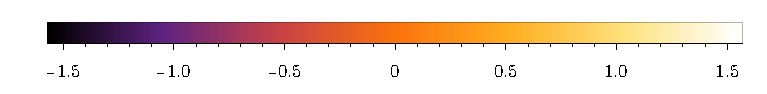
\includegraphics[scale=1.2]{../img/N=3_barA.pdf}
    \caption{Arctangens of the metric tensor for higher state manifolds. By  rows: $M_0$, $M_1$; $M_2$, $M_3$; $M_4$, $M_5$.}
    \label{fig:higherStateManifolds}    
\end{figure}


\begin{figure}[H]
    \centering
    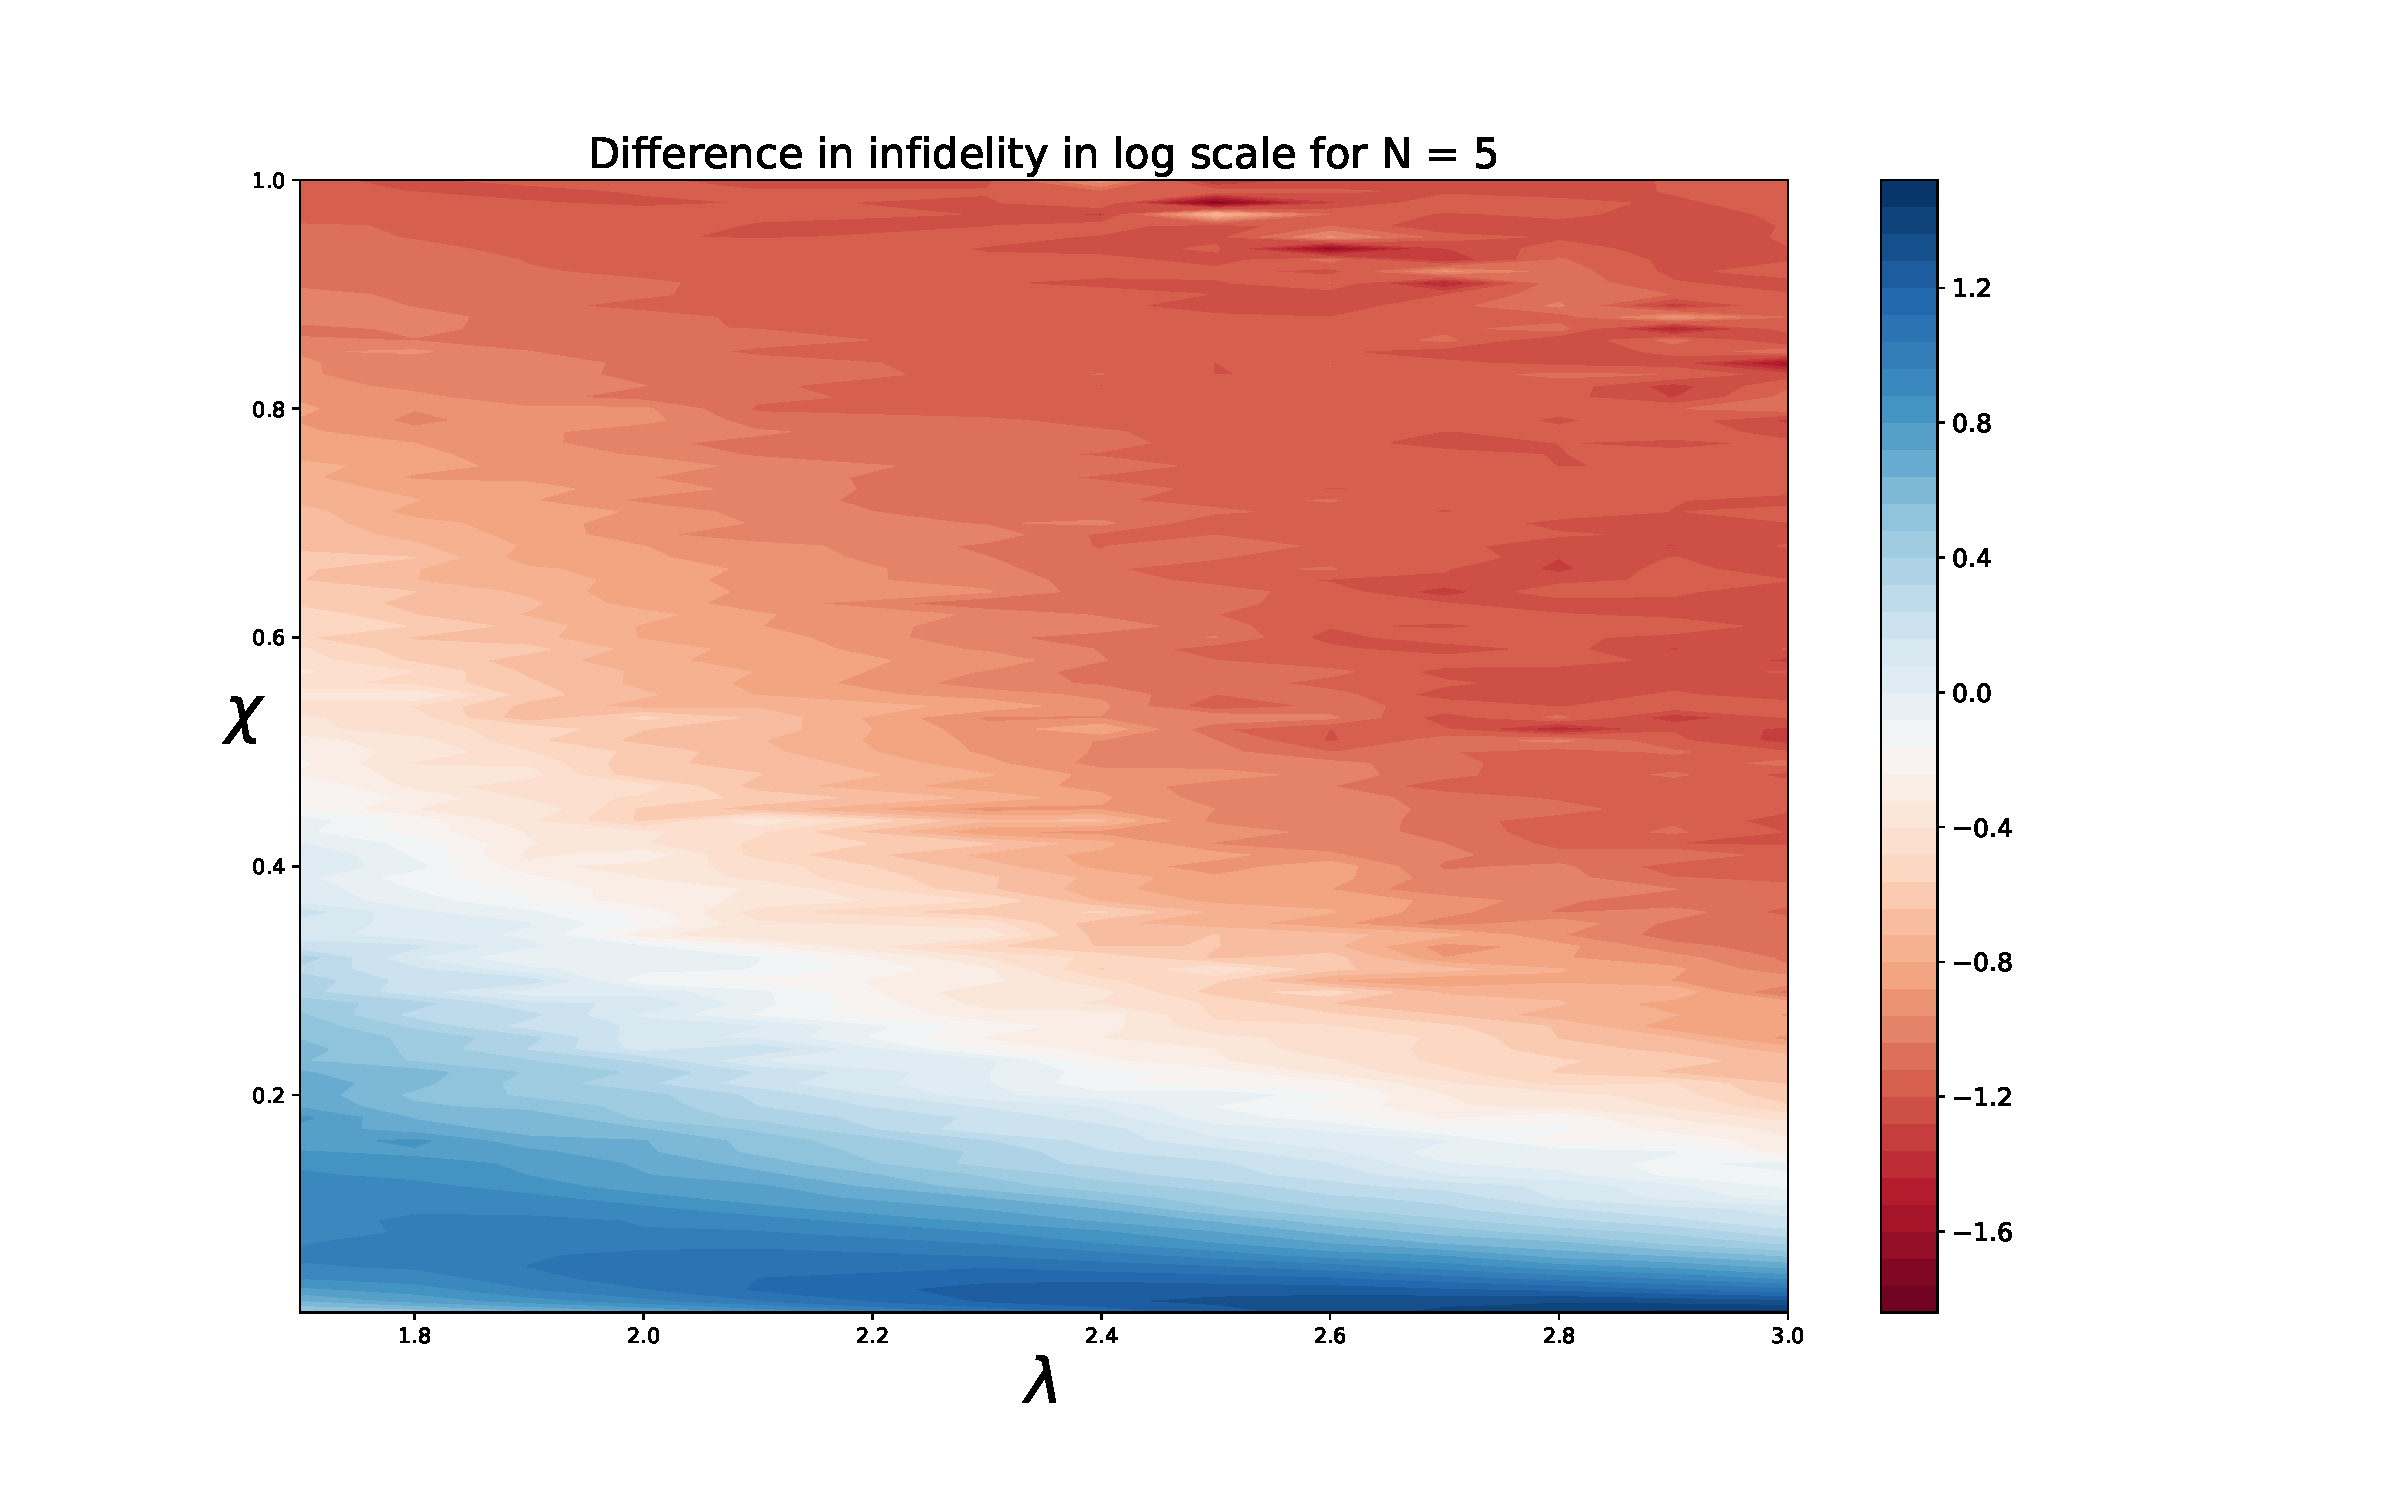
\includegraphics[width=1\textwidth]{../img/fidelity_lineVSgeodesic.pdf}
    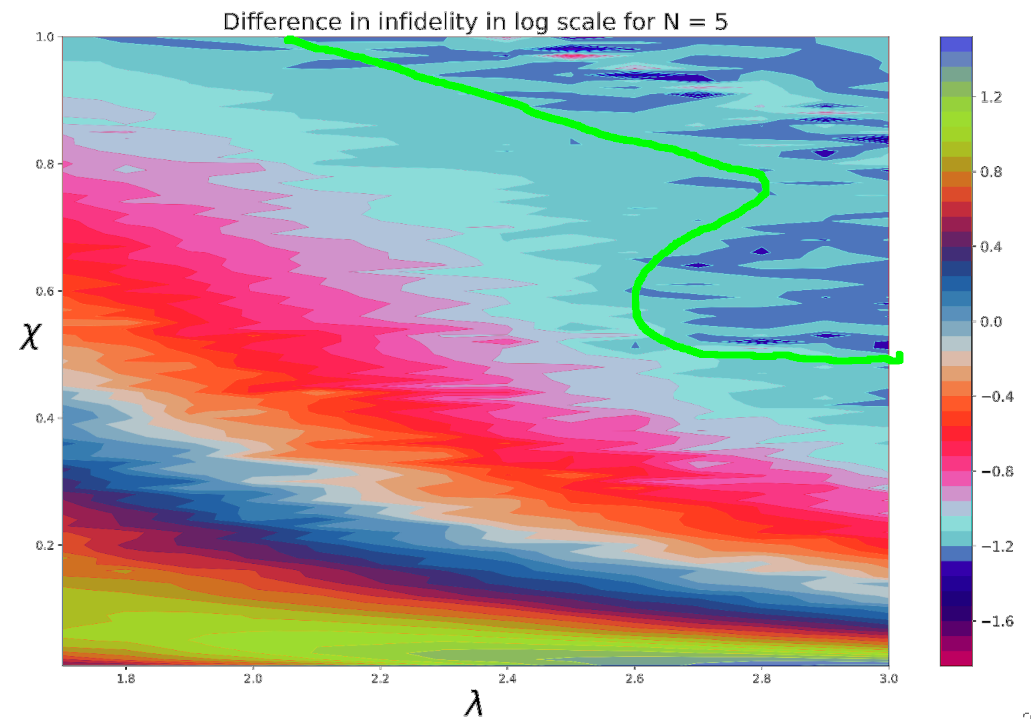
\includegraphics[width=0.8\textwidth]{../img/fidelity_geodesicVSline_fuckedupcolors.png}
    \caption{\textcolor{gray}{Infidelity difference between line and geodesic, above picture is original from Felipe, bottom one is edited in GIMP to see the difference more clearly.}}
    \label{fig:higherStateManifolds}    
\end{figure}
